\documentclass[letter,openrigh,12pt,spanish]{report}
%Gummi|065|=)
\title{\textbf{Identificar las aplicaciones de los manipuladores paralelos}}
\author{Diego Armando Becerra Iñiguez\\
		Cinem\'atica de Robots\\
		Ing. Mecatr\'onica 7to A}
\date{1 de noviembre de 2019}
\usepackage{graphicx}
\begin{document}

\maketitle

\section{Aplicaciones de los robots paralelos}

La principal ventaja de los robots paralelos viene por la capacidad de distribuir las cargas aplicadas sobre el elemento terminal entre las piernas o cadenas cinem\'aticas abiertas que unen la plataforma m\'ovil a la plataforma base. Es as\'i como las cadenas cinem\'aticas o piernas le proporcionan una mayor rigidez al robot. Sin embargo, las piernas limitan si espacio de trabajo por las restricciones que introducen la configuracion de cadena cerrada. Esto se explica haciendo un s'imil con el cuerpo human, una cadena cinem\'atica abierta (robot serial) puede ser vista como un solo brazo con el que se pueden realizar diversas tareas. Sin embargo, si se requiere de mayor fuerza o de precisi\'on el ser humano emplea los dos brazos. CUando se utilizan los dos brazos para manipular una pieza se est\'a usando el concepto de robot paralelo teniendo en cuenta que la base fija es el toroso y la plataforma m\'ovil equivale al elemento sujetado con ambas manos. Siguiendo este s\'imil, se puede observar que con los dos brazos se gana mayor capacidad de carga, mayor precisi\'on pero a expensas de perder espacio de trabajo.

A pesar de la desventaja de poco espacio de trabajo. Sus ventajas comparativas con respecto a los robots seriales que desde su aparici\'on a mediados de los 50, cada d\'ia se desarrollen m\'as aplicaciones en el sector industrial y en nuevos campos como la rob\'otica de servicio. 

\subsection{Aplicaciones iniciales}

Un robot paralelo consiste de una plataforma m\'ovil unida a una plataforma fija mediante una serie de cadenas cinem\'aticas llamdas piernas, Partiendo del anterior concepto, Bonev estable que el origen del robot paralelo se encuentra en la industria del entretenimiento, siendo James E. Gwinnett en el año 1928 uno de los pioneros en patentar un artefacto basado en el concepto de robot paralelo. La \ref{Figura 1} presenta una esquema incluido en el documento de la patente original. El dispositivo presenta una arquitectura donde una cadena cinem\'atica o pierna central restringe movimiento de la plataforma m\'ovil respecto a la base de forma tal que su movimiento resultante es del tipo esf\'erico. Una cadena cin\'ematica ubicada en uno de los extremos de las plataformas, provee el movimiento de rotaci\'on a la plataforma m\'ovil que se aprovechado para producir el moviento requerido para el entretenimineto de los usuarios.

\begin{figure}[htp]
\centering
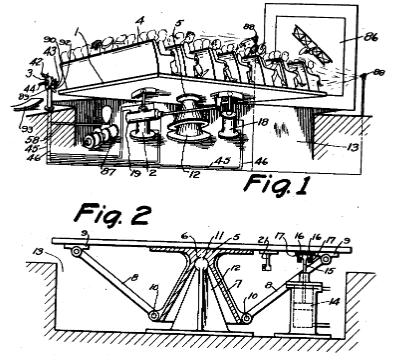
\includegraphics[width=8cm]{fi2.png}
\caption{}
\label{Figura 1}
\end{figure}

La primera aplicacion industrial conocida del robot paralelo, fue presentanda por Willard L. V. Pollard en el año 1940. El dispositivo fue propuesto para pintar veh\'iculos de forma autom\'atica con pintura de aerosol y posteriormente fue pantentado como dispositivos para controlar el posicionamiento de una herramiento. La \ref{Figura 2} muestra una representaci\'on esquem\'atica del ingenieso aparato de 5 grados de libertad (GDL) donde la plataforma m\'ovil va unida a la fija mediante 3 cadenas cinem\'aticas o piernas. El dise\~no presenta tres motores que determinan la posici\'on de la cabeza de la herramienta, y de otroso dos motores que mediante un sistema de cables transmite el movimiento que permite orientar la herramienta.

\begin{figure}[htp]
\centering
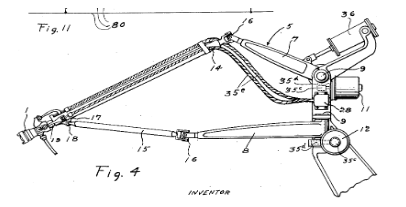
\includegraphics[width=8cm]{fi1.png}
\caption{}
\label{Figura 2}
\end{figure}

M\'as tarde en la d\'ecada de los 50, Eric Gough un ingeniero automotriz trabajando en la f\'abrica de neum\'aticos de la Ford Dunlop en Birmingham, INglaterra, desarrola una m\'aquina Universal de pruebas de neum\'aticos. La plataforma fue puesta en funcionamiento en el a\~no 1954 y cumpl\'ia la funci\'on de probar mec\'anicamente neum\'aticos mediante la aplicaci\'on de cargas combinadas. La \ref{Figura 4} muestra una imagen del dispositivo utilizado por la empresa Dunlop hasta el cierre de la f\'abrica en el a\~no 1980. SU dise\~no preenta una forma de octaedro donde cada cinem\'atica es impulsada por actuadores lineales. EL mecanismo presneta 6 GDL.


\begin{figure}[htp]
\centering
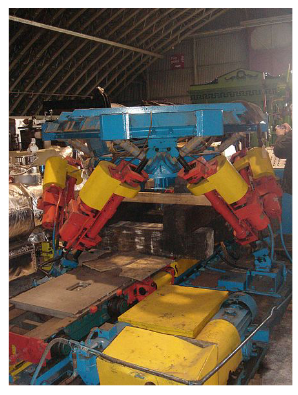
\includegraphics[width=8cm]{fi5.png}
\caption{}
\label{Figura 4}
\end{figure}

Stewart introduce un robot paralelo de 6 GDL similar al de Gough. debido al parecido que presenta la plataforma Stewart con el robot propuesto por Gough hoy en d\'ia la configuraci\'on del tipo hex\'apodo con actuadores lineales se conoce como plataforma Gough-Stewart. Es de destacar que la plataforma Stewart fue porpuesta para aplicaciones de simulador de vuelo. La \ref{Figura 3} muestra el robot basado en el concepto de Stewart desarrolaldo para un simulador de vuelo de Lufthansa. Es justo tambi\'en indicar que Klaus Cappel en 1964 de forma separada. y sin tener conocimiento previo de los trabajos de Gough y de Stewart, patenta una configuraci\'on similar al robot hex\'apodo como dispositivo para simulaci\'on de movimiento.

\begin{figure}[htp]
\centering
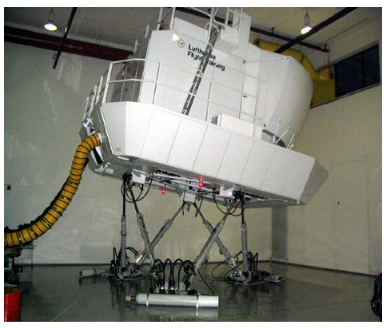
\includegraphics[width=8cm]{fi3.png}
\caption{}
\label{Figura 3}
\end{figure}

Los robots anteriores representan las palicaciones iniciales de los robots paralelos, pero no es hasta el a\~no 1987 que los robots paralelos vuelven a tener un auge en la comunidad cientifica y de desarrollo de aplicaciones.

\subsection{Aplicaciones de Pick and Place (Recoger y Colocar)}

La palicaci\'on m\'as conocida y desarrolada de estos robots es en operaciones de \textit{pick and place}. Es de destacar que el robot serial equivale para este tipo de operaciones lo constituye el robot SCARA (Selective Compliant Assembly Robot Arms) que presenta 4 GDL. Un robot SCARA permite posicionar el elemento terminal, y por ende la pieza, en el espacio cartesiano, adem\'as tambi\'en puede realizar una rotaci\'on. A este tipo de movimiento se le conoce como movimientos de Schoenflies. El primer robot comercial y posiblemente uno de los m\'as exitososo en implementaci\'on industrial lo constituye el robot Delta desarrolado a partir de la dec\'ada de los 80 en la Ecole Polytechnique Federale de Lausanne, SUiza por Reymond Clavel. El robot fue desarrollado partiendo de la idea de desarrollar un robot para manipuar objetos de bajo peso a altas velocidades. La particularidad del robot Delta es que la plataforma m\'ovil va unida a la base mediante 3 piernas donde cada pierna presenta un mecanismo de paralelogramo que permite balancear el centro de masa de cada uno de ellas. Las piernas se unen a la base fija mediante pares o juntas universales (U). La \ref{Figura 5} muestra la representaci\'on esquem\'atica del robot Delta donde el movimiento en el espacio. Generalmente la plataforma superior va fija a la bancada, mientras que la plataforma inferior es la m\'ovil donde va ubicado la herramiento.

\begin{figure}[htp]
\centering
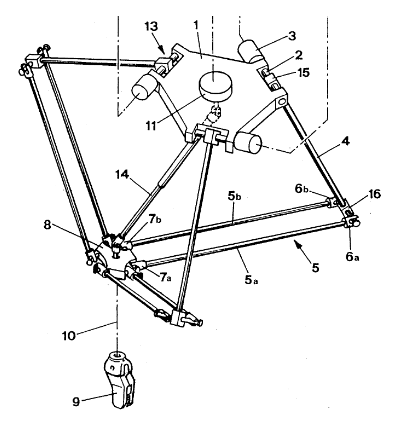
\includegraphics[width=8cm]{fi4.png}
\caption{}
\label{Figura 5}
\end{figure}

\subsection{Aplicaciones en centro de mecanizado}

otra de las aplicaciones pr\'acticas de los robots paralelos se encuentran en el \'area de desarrollo de centros de mecanizado. En este campo es com\'un que los desarrolladores se refieran al robot paralelo como Mecanismo Cinem\'atico Paralelo (MCL) en ingl\'es Paralle Kinematic Mechianism (PKM). El primer prototipo de centro de mecanizado basado en la en MCP fue presentado al p\'ublico en el evento Inernational Manifacturing Technology Show (IMTS) de 1994 en Chicago, USA. EL dispositivo utiliza un robot paralelo del tipo plataforma Stewart (6 GDL) para realizar operaciones de mecanizado en 5 ejes. A partir su introducci\'on en 1994 el n\'umero de desarrollo y patentes de centros de mecanizado basados en MCP ha incrementedo constantemente.

\subsection{Aplicaciones en la cirug\'ia rob\'otica}

La cirug\'ia minimamente invasiva representa una de las \'areas donde la intrpducci''on de robot produce un gran impacto, sobre todo mejorando las presentaciones dee la cirug\'ia laporosc\'opica, ya que aumenta la habilidad del cirujano a la hora de realizar una operaci\'on (mayor precisi\'on, evitar el movimiento err\'atico del pulso de la mano). Con la cirug\'ia rob\'otica se han logrado avances como realizar una operaci\'on mediante orificios de 10 mm en el cuerpo del paciente. En la actualidad solo hay un robot comercial disponible que es el sistema Da Vinci. EL sistema se ha comercializado a partir de los a\~nos 90 y en el a\~no 2000 fue autorizado por la Administraci\'on de alimentos y Medicamento (FDA) de los Estados Unidos. El robot consiste de 3 o 4 brazos rob\'oticos del tipo se\~nal, una consola o monitor para interacci\'on del m\'edico con el robot y una camilla donde se ubica al paciente.

\subsection{Aplicaciones en rob\'otica para rehabilitaci\'on}

La rehabilitaci\'on se presenta como otro de los campos de mayor inter\'es en la actualidad sirviendo de asistencia al trabajo arduo de los fisoterapeutas, adem\'as de que logra una mejor coordinaci\'on para los ejercicios de rehabilitaci\'on y mayor precisi\'on en el diagn\'ostico de lesiones y la medici\'on de la evoluci\'on de los pacientes. La rehabilitaci\'on y giagnosis de las extremidades inferiores es muy frecuente debido a la gran cantidad de accidentes a los que est\'an expuestas estas extremidades de hecho, en el campo de los deportes suelen presentarse muy a menudo.

\subsection{Aplicaciones en el laboratorio UPV y Mecabot-Ula}

El Laboratorio de Mecatr\'onica y Rob\'otica de la Universidad de los Andes (MECABOT-ULA), Venezuela, conjuntamente con grupos de investigaci\'on de la Universidad Politecnica de Valencia han venido desarrollando metodolo\'ias para el dise\~no de sistemas biomecatr\'onicos para el diagnostico y rehabilitaci\'on de extremidades del cuepro humano. En particular, se han desarrolado y construido dos prototipos rob\\oticos para rehabilitaci\'on de la extemidad inferior.

\begin{thebibliography}{x}
\bibitem{Anual} \textit{Aplicaci\'on de los robots Paralelos} Miguel D\'iaz Rodriguez \textsc{HAL} primera edici\'on 13 Nov 2018 
\end{thebibliography}

\end{document}
